%!TEX root = Manuscrit.tex
\chapter{Segmentation sémantique multi-modale}
\label{chap:multimodal}

\chapsummary{%
Nous avons vu dans les chapitres précédents que les réseaux de neurones entièrement convolutifs permettaient d'établir de nouveaux états de l'art en segmentation sémantique d'images de télédétection et ce y compris pour des capteurs non-conventionnels. Toutefois, nous avons souligné la difficulté d'obtenir des résultats satisfaisants avec des sources de données n'offrant qu'une information partielle, comme le \gls{Lidar}.

Dans ce chapitre, nous investiguons des méthodes de fusion de données permettant d'exploiter en simultanée plusieurs capteurs. Nous proposons ainsi plusieurs architectures de réseaux de neurones multi-modales capables de traiter en parallèle des données hétérogènes, comme les modèles numériques de terrain et les images optiques. Nous validons ces modèles avec succès sur plusieurs jeux de données et montrons qu'il est possible de tirer ainsi profit de la complémentarité des différents capteurs.

Nous étendons ensuite ces travaux à des sources de données non physiques. En particulier, nous étudions la possibilité d'intégrer de l'information sémantique \emph{a priori} venant de bases de données géographiques en ligne pour consolider les cartes sémantiques prédites par le réseau. En traitant ces données comme un nouveau capteur virtuel, nous pouvons ainsi utiliser nos architectures multi-modales profondes pour injecter de l'information connue dans le processus d'apprentissage et d'inférence de nos réseaux de neurones.
}

\section{Apprentissage multi-modal}

\subsection{Approches en vision par ordinateur}

Principalement autour du RGB+profondeur

Empilement ne donne rien

Approches de fusion a posterio, par exemple auto-encodeurs audio/vidéo

Approches d'apprentissage conjoint, par exemple FuseNet

L'apprentissage profond a été étudié à plusieurs reprises pour le traitement de données multi-modales. \citet{ngiam_multimodal_2011} ont proposé une architecture d'auto-encodeur à double entrée apprenant une représentation conjointe des sources audio et vidéo. Dans la communauté vision, la popularisation des capteurs \gls{RGB-D} comme la Kinect a entraîné de nombreux travaux en interprétation de scènes utilisant à la fois les images et les cartes de profondeur. Ainsi, \citet{eitel_multimodal_2015} introduit une architecture de réseau profond dérivée d'AlexNet utilisant deux réseaux convolutifs parallèles convergeant une représentation mixant image \gls{RVB} et carte de profondeur encodée sur trois canaux pour la classification d'images. Cette approche de réseaux parallèles convergeant vers une représentation mixte a également été appliquée à la détection d'extremités des doigts par~\citet{guo_two-stream_2016}.
Plus récemment, \citet{hazirbas_fusenet_2016} ont étendu cette idée aux réseaux entièrement convolutifs pour la segmentation sémantique d'images \gls{RGB-D} en utilisant un SegNet avec deux encodeurs parallèles dont les représentations intermédiaires régulièrement combinées. Finalement, \cite{lee_rdfnet_2017} élabore ce modèle en y intégrant de l'apprentissage par résidu et une approche de segmentation par raffinement des cartes sous-résolues. Ces différents modèles permettent de fait d'extraire de l'information à partir de sources de données hétérogènes, mais toutefois se focalisent sur des images traditionnelles.

\subsection{Transposition à la télédétection}

\todo[inline]{Marmanis, etc., état de l'art fusion en télédétection}

\begin{figure}
  \begin{subfigure}{0.5\textwidth}
    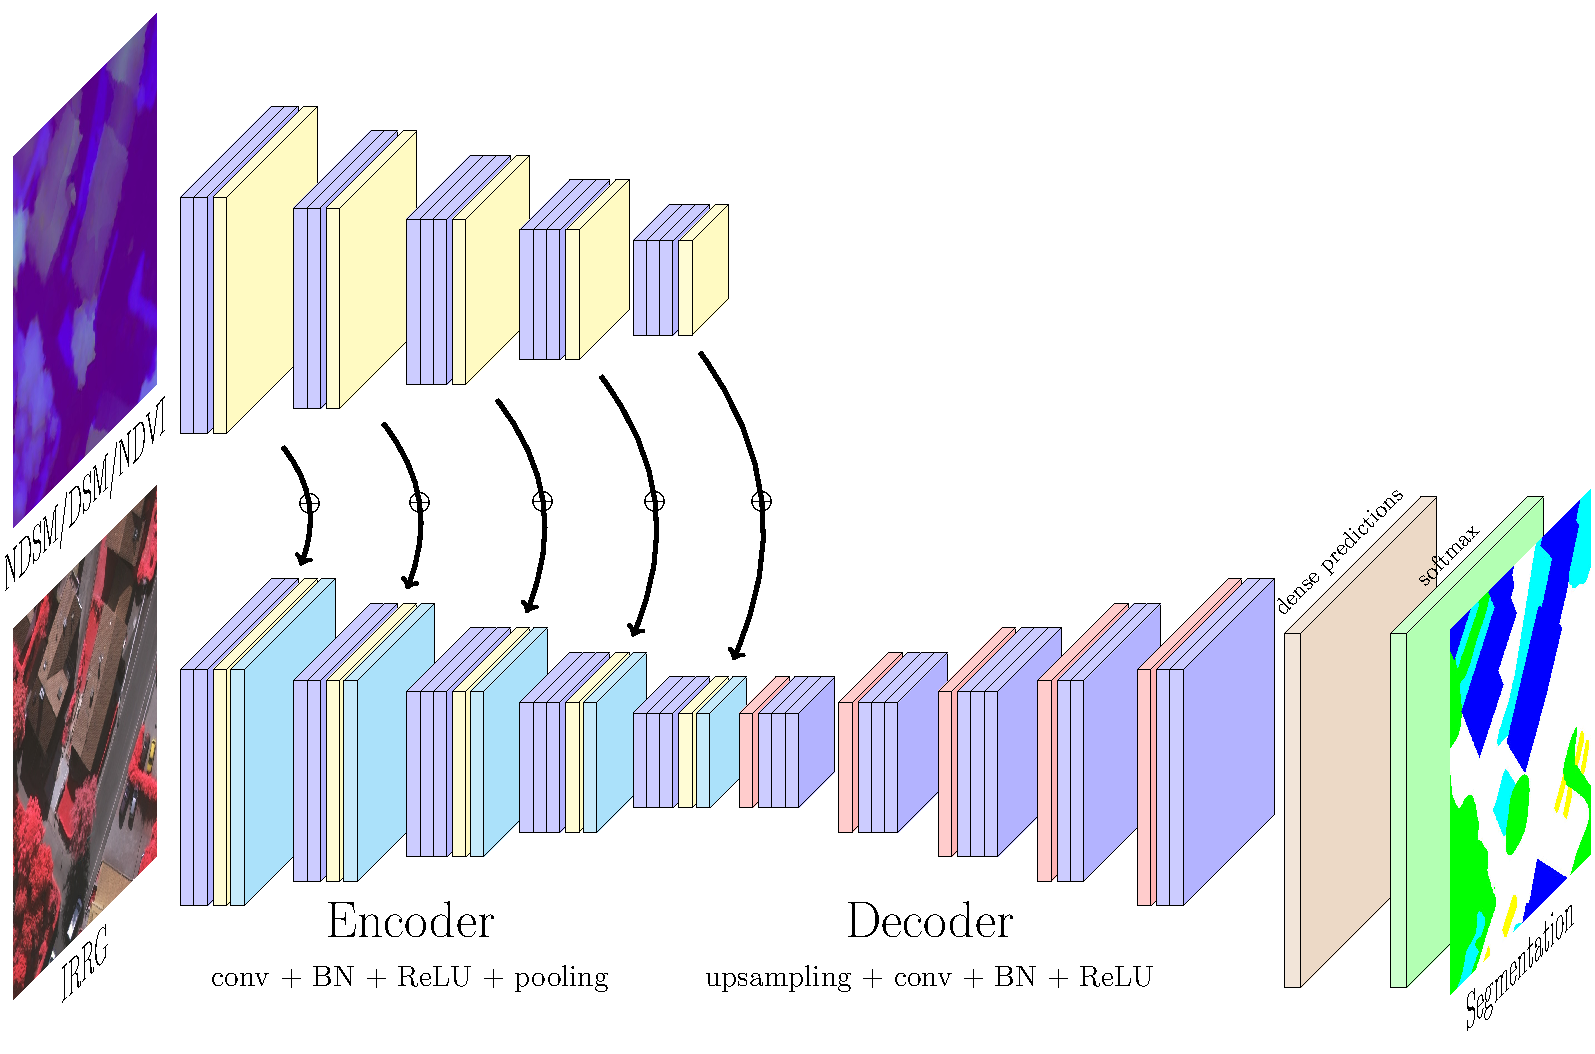
\includegraphics[width=\textwidth]{fusenet}
    \caption{Architecture FuseNet~\cite{hazirbas_fusenet_2016}}
    \label{fig:fusenet}
  \end{subfigure}%
  \begin{subfigure}{0.5\textwidth}
    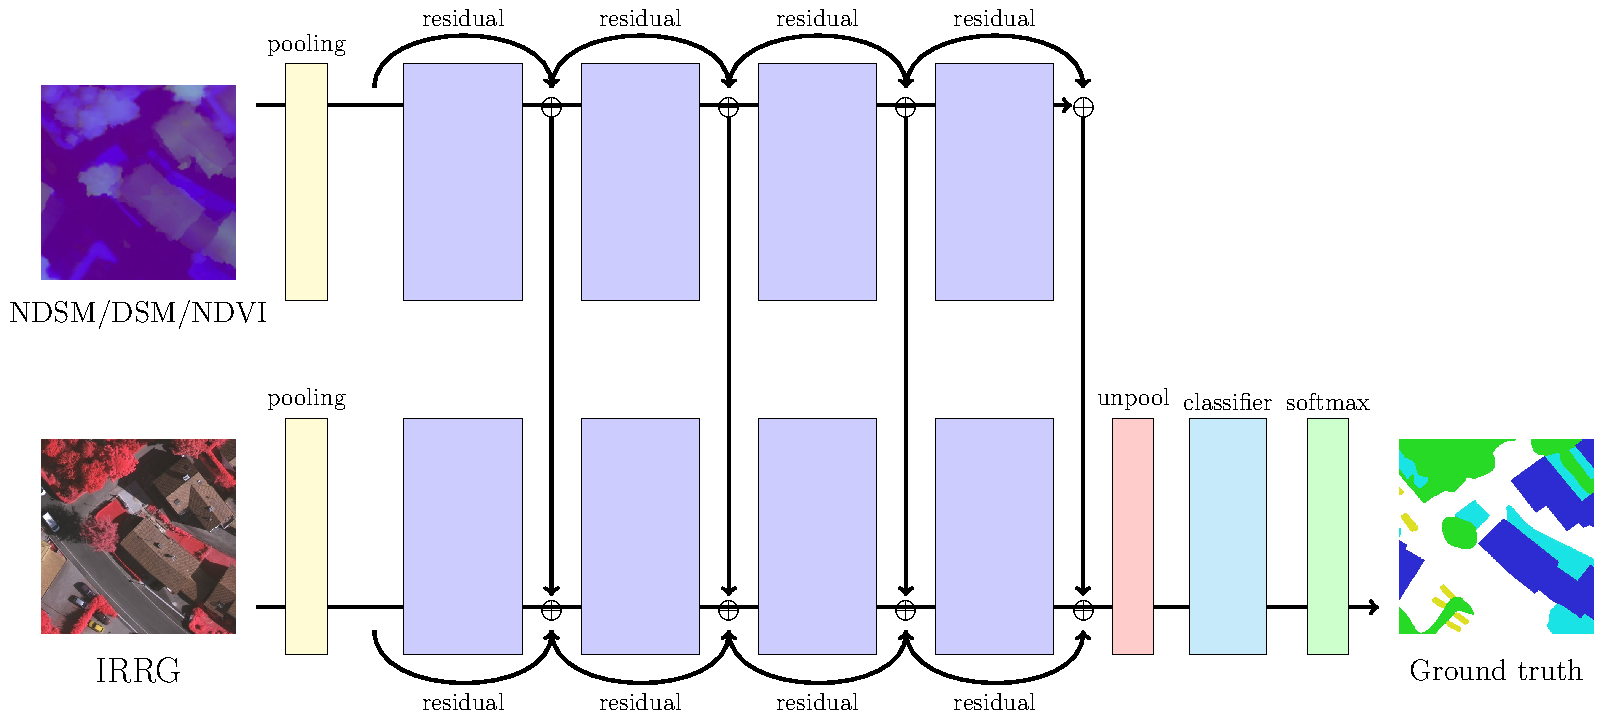
\includegraphics[width=\textwidth]{fusresnet}
    \caption{Architecture FuseResNet}
    \label{fig:fusresnet}
  \end{subfigure}
\end{figure}

Ces images \gls{RGB-D} correspondent à une représentation 2,5D du monde. L'approche FuseNet~\cite{hazirbas_fusenet_2016} est dérivée de l'architecture SegNet. Comme illustré dans la~\cref{fig:fusenet}, FuseNet encode conjointement l'image \gls{RVB} et la carte de profondeur en utilisant deux encodeurs dont les contributions respectives sont additionnées après chaque bloc convolutif. Un décodeur unique réalise alors la reconstruction de la résolution et la classification. Cette approche peut être adaptée à n'importe quel autre \gls{CNN} de base, comme les ResNet (cf.~\cref{fig:fusresnet}).

Dans notre cas, nous pouvons altérer FuseNet de la même façon que nous avons altéré SegNet dans les chapitres précédents, afin de traiter des images de télédétection. En effet, une carte d'élévation comme le \gls{MNE} peut être considérée comme une carte de profondeur associée à une image \gls{RVB}. De fait, nous proposons ainsi d'adapter FuseNet au traitemement d'images de télédétection multi-modales, exploitant à la fois l'image optique, mais aussi l'image composite conçue au chapitre précédent.

%However, in this architecture the depth data is treated as second-hand. Indeed, the two branches are not exactly symmetrical: the depth branch works only with depth-related information where as the optical branch actually deals with a mix of depth and optical data. Moreover, in the upsampling process, only the indices from the main branch will be used. Therefore, one needs to choose which data source will be the primary one and which one will be the auxiliary data~(cf.~\cref{fig:fusenet_sum}). There is a conceptual unbalance in the way the two sources are dealt with. We suggest an alternative architecture with a third ``virtual'' branch that does not have this unbalance, which might improve performance.

%Instead of computing the sum of the two sets of feature maps, we suggest an alternative fusion process to obtain the multi-modal joint-features. We introduce a third encoder that does not correspond to any real modality, but instead to a virtual fused data source. At stage $n$, the virtual encoder takes as input its previous activations concatenated with both activations from the other encoders. These feature maps are passed through a convolutional block to learn a residual that is summed with the average feature maps from the other encoders. This is illustrated in~\cref{fig:fusenet_mix}. This strategy makes FuseNet symetrical and therefore relieves us of the choice of the main source, which would be an additional hyperparameter to tune. This architecture will be named \textbf{V-FuseNet} in the rest of the paper for Virtual-FuseNet.

\section{Fusion de modèles}

\subsection{Mélanges de modèles}

Approches a posteriori : moyenne ou combinaison apprise

Similaire à de l'apprentissage par ensemble

\subsection{Fusion par apprentissage}

Un des inconvénients de FuseNet est que cette approche nécessite d'avoir des modèles de base topologiquement compatible afin de pouvoir sommer les activations et fusionner les encodeurs. Cependant, cela ne se vérifie pas systématiquement. Par exemple, certaines données peuvent posséder des natures différentes, comme une image 2D et un nuage de point 3D. En outre, il n'est pas nécessairement utile de consacrer autant de paramètres sur les deux sources de données, notamment si l'une est moins informative que l'autre. Nous proposons donc une méthode de fusion de données alternative pour extraire de l'information à partir de sources hétérogènes. En l'occurrence, nous suggérons d'étudier la posibilité d'effectuer une fusion tardive au moment de la prise de décision, plutôt que d'apprendre des représentations conjointes.

\begin{figure}
   \begin{subfigure}{0.5\textwidth}
     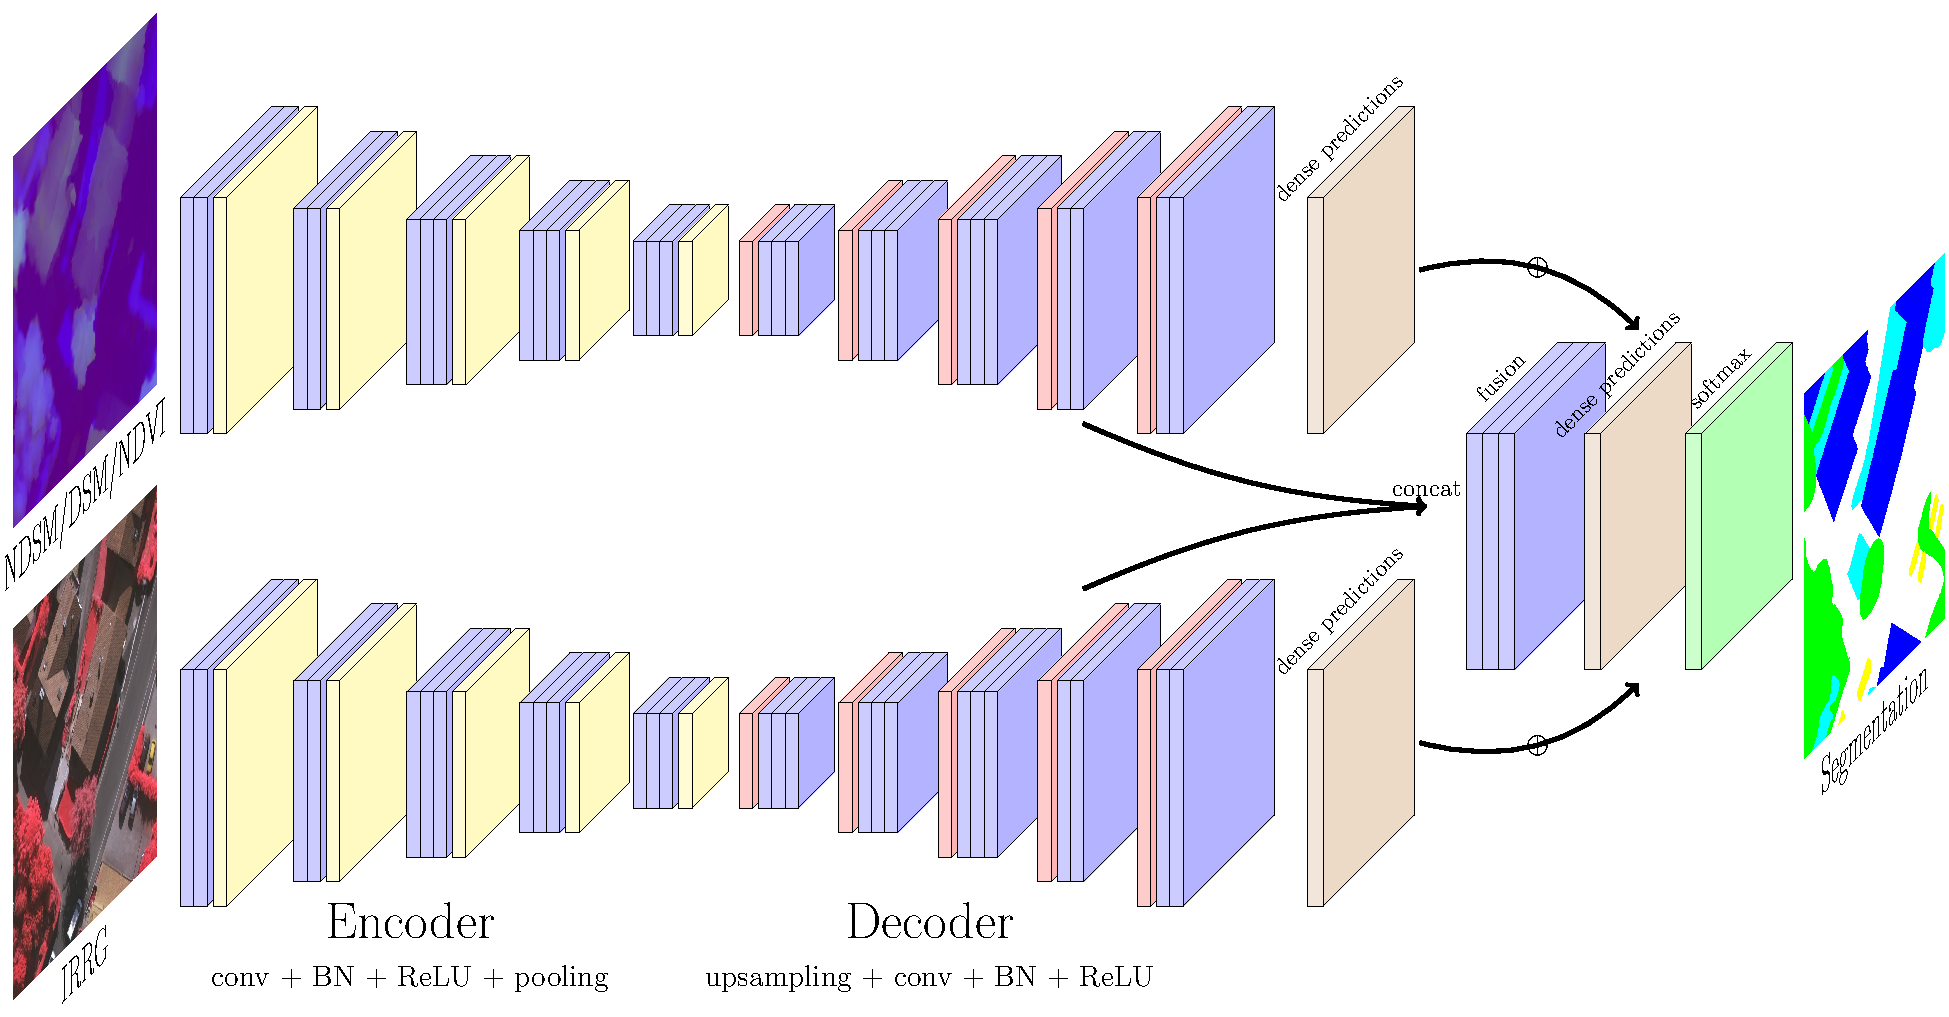
\includegraphics[width=\textwidth]{residual_fusion_segnet}
     \caption{Correction résiduelle appliquée à SegNet}
     \label{fig:residual_correction}
   \end{subfigure}
   \begin{subfigure}{0.5\textwidth}
     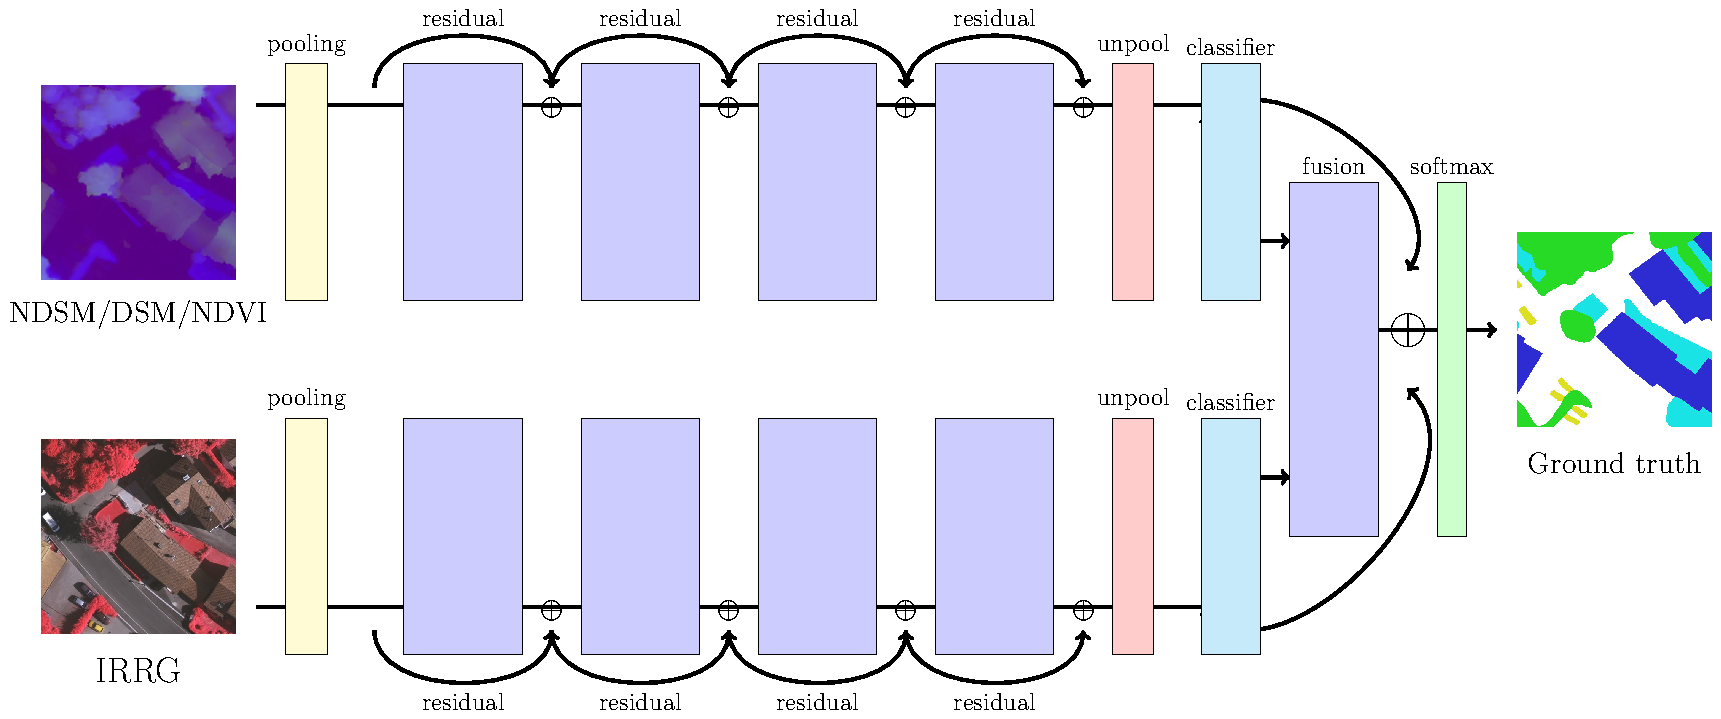
\includegraphics[width=\textwidth]{resnet_rc}
     \caption{Correction résiduelle appliquée à ResNet}
     \label{fig:residual_correction_resnet}
   \end{subfigure}
\end{figure}

Par exemple, il est envisageable d'entraîner un modèle par modalité et de réaliser la moyenne des prédiction. Toutefois, cela ne permet pas de prendre en compte les particularités de chaque capteur. Nous introduisons donc un module de correction résiduel qui prend en entrée les dernières cartes d'activation des réseaux et réalise une fusion des cartes de probabilités~\cite{audebert_semantic_2016}. Le module de correction résiduel apprend la correction $\epsilon$ à appliquer à la prédiction moyenne pour améliorer les performances globales du modèle combiné. Ce processus est illustré dans la~\cref{fig:residual_correction} pour SegNet et dans la~\cref{fig:residual_correction_resnet} pour ResNet.

Building on the idea of residual deep learning~\cite{he_deep_2016}, we propose a fusion network based on residual correction. We define a convolutional residual block using the same parameters as the rest of the SegNet network ($3\times3$ convolutions and $1$ pixel of padding). Intermediate feature maps from the decoding parts of the two SegNets are fed as inputs to a 3-convolution layers ``correction'' network (cf. \cref{fig:residual_correction}. The output of the residual block is then summed in the residual fashion with the average of the two predictions, as illustrated by \cref{fig:residual_correction}. Residual learning fits this use case, as the average score is already a close estimate of the truth. To improve the results, we aim to use the complementary channels to correct small errors in the prediction maps. In this context, the residual can be seen as a corrective term for our predictive model. This module is trained using backpropagation on the standard softmax loss. Learning rates for the input SegNets are set to zero, as this considerably speeds up the training without significant loss.

%Let $M_r$ denote the input of the $r^{th}$ stream ($r \in \{1,\dots,R\}$ with $R = 2$ here), $P_{r}$ the output probability tensor and $Z_r$ the intermediate feature map used for the correction. The corrected prediction is:

% \begin{equation}
% P'(M_1, \dots, M_R) = P(M_1, \dots, M_R) + correction(Z_1, \dots, Z_R)
% \end{equation}
% where
% \begin{equation}
% P(M_1, \dots, M_n) = \frac{1}{R}\sum_{r=1}^R P_r(M_r)~.
% \end{equation}

En notant $P_0$ le tenseur représentant la vérité terrain, $P_i$ les prédictions pour la $i$\ieme sortie\,:
\begin{equation}
P_i = P_0 + \epsilon_i \text{ where } \lvert \epsilon_i \lvert  \ll \rvert P_i \rvert
\end{equation}

$\epsilon_i$ est un terme d'erreur, petit tant que la prédiction $P_i$ est suffisamment exacte. Le module de correction résiduelle doit donc apprendre à estimer l'erreur et à inférer les cas où elle apparaît ainsi que comment la corriger.

Si $R$ est le nombre de prédictions sur lesquelles réaliser la correction résiduelle, alors le module prédit $P'$, la somme des prédictions moyenne et de la correction $c$ :
\begin{equation}
P' = P_{avg} + c = \frac{1}{R} \sum_{i=1}^R P_i + c = P_0 + \frac{1}{R} \sum_{i=1}^R \epsilon_i + c
\end{equation}

Le module de correction résiduel étant optimisé pour minimiser la fonction de coût, cette contrainte impose\,:
\begin{equation}
\lVert P' - P_0 \rVert \rightarrow 0
\end{equation}
ce qui impose la contrainte suivante sur $c$ et $\epsilon_i$\,:
\begin{equation}
\lVert \frac{1}{R} \sum_{i=1}^R \epsilon_i - c \rVert \rightarrow 0
\end{equation}

\begin{figure}[t]
  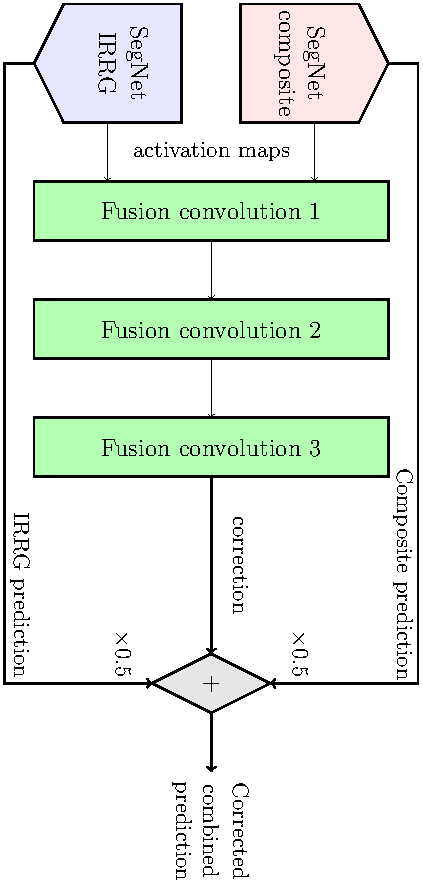
\includegraphics[height=\textwidth,angle=90]{correct_network}
  \caption{Module de correction résiduelle.}
  \label{fig:correction_network}
\end{figure}

De fait, cela peut se traduire par l'approximation de l'erreur moyenne en fonction des cartes d'activation finales. En effet, lors de la phase d'entraînement, la vérité terrain $P_0$ est connue et le module de correction résiduel est modifié afin de se rapprocher de $\sum_{i=1}^R \epsilon_i$. L'apprentissage par résidu se prête tout particulièrement à cette approche, car celle-ci s'exprime naturellement sur la forme d'une correction d'erreur, le résidu étant alors de faible amplitude par rapport au signal identité (ou \emph{bypass}). Le module est détaillé dans la~\cref{fig:correction_network}.

Laisser le modèle trouver la combinaison intéressante : ~moyenne avec pondération adaptative

Approche résiduelle : correction d'erreur

\section{Connaissances \textit{a priori}}

\subsection{OpenStreetMap}

Présentation d'OSM
\glsfirst{OSM} est un \gls{SIG} libre et participatif alimenté par un ensemble de contributeurs bénévoles qui cartographient leurs environs. Les contributeurs peuvent utiliser l'éditeur en ligne pour annoter des fonds de carte géoréférencés en y ajoutant ou en mettant à jour les éléments du réseau routier, les empreintes au sol des bâtiments, les espaces verts, etc. En plus de ces éditions manuelles, la communauté \gls{OSM} utilise certaines sources de données officielles, comme le cadastre de l'État français afin de mettre à jour les limites administratives des entités géographiques ou pour importer les nouveaux bâtis. Le principal intérêt d'\gls{OSM} est qu'il s'agit de la plus grande base de données d'information géographique sous licence libre au monde. La base de données contient des informations sur une large taxonomie d'entités géographiques, allant des autoroutes aux parcs de loisir en passant par les églises, les cimetières ou les parcelles agricoles.

Peu de travaux se sont penchés sur l'intégration des données \gls{OSM} pour l'apprentissage automatique depuis l'ouverture du site en 2004. Le plus souvent, \gls{OSM} est utilisée comme vérité terrain pour la détection de routes et de bâtiments~\cite{mnih_machine_2013,maggiori_learning_2017} dans un contexte d'apprentissage supervisé ou pour le recalage automatique d'images satellites~\cite{vakalopoulou_simultaneous_2016}. \citet{isola_image--image_2016} se sont intéressés à la génération automatique de tuiles \gls{OSM} à partir d'images satellites, mais seulement à des fins visuelles, sans évaluation selon des métriques de classification. Pourtant, \gls{OSM} est une source de données riche permettant d'extraire de l'information géographique sémantique de haut niveau. \citet{chen_deepvgi_2017} ont de fait utilisé des méthodes d'apprentissage actif pour détecter automatiquement les objets non encore présents dans \gls{OSM} afin de les suggérer aux contributeurs. \citet{danylo_contributing_2016} ont utilisé des forêts aléatoires appliquées sur certaines couches de données \gls{OSM} pour prédire des zones climatologiques locales, tandis que \citet{geis_joint_2017} se sont penchés sur la détection automatique de zones sujettes à des catastrophes naturelles.

Ici, nous suggérons d'utiliser les couches sémantiques d'\gls{OSM} comme entrée à un réseau de neurones profond pour la cartographie automatisée. L'idée est d'exploiter la donnée sémantique, possiblement bruitée et incomplète d'\gls{OSM} afin d'extraire de l'information plus riche à une résolution supérieure.

Pour ce faire, nous considérons le jeu de données ISPRS Potsdam sur lequel nous récupérons les données \gls{OSM} de 2017. Nous sélectionnons les couches correspondant aux routes, aux empreintes de bâtiments, aux zones d'eau et aux espaces verts. Les routes sont définies dans \gls{OSM} comme un réseau filaire. Par conséquent, en fonction du type de route indiqué dans \gls{OSM}, nous assignons une largeur arbitraire à celles-ci. En outre, les bâtiments, espaces verts et zones d'eau ne correspondent pas nécessairement entièrement aux images aériennes du jeu de données, soit à cause de constructions nouvelles (les images ont été acquises en 2014) , soit car les annotations \gls{OSM} sont incomplètes par endroits. Nous générons ainsi un raster à la même résolution que les images \gls{RVB} contenant 4 canaux binaires : un pour le masque des routes, un pour les bâtiments, un pour l'eau et un pour les espaces verts.

\subsection{Information \textit{a priori} comme capteur virtuel}

L'idée de notre approche est de traiter le raster \gls{OSM} ainsi formé comme un capteur virtuel, c'est-à-dire comme une source de données complémentaire aux images optiques. Le raster ainsi formé contient une information partielle et incomplète, mais pouvant néanmoins faciliter le travail du réseau profond. En effet, plutôt que d'apprendre à reconnaître un bâtiment uniquement à partir de l'image optique, un réseau muni des deux sources de données peut se reposer en partie sur les annotations \gls{OSM} pour repérer les bâtiments, et consacrer une partie de ses poids à gérer d'autres cas de figure plus difficiles.

Nous appliquons donc les méthodes de fusion de donnée FuseNet et de correction résiduelle en utilisant comme entrées les images optiques et les couches \gls{OSM}.

Lorsque les classes d'intérêt de la segmentation sémantique sont déjà présentes dans les données OSM, comme pour les bâtiments ou les routes, il est possible de les utiliser comme premières approximations de la vérité terrain. Celles-ci pourront ensuite être raffinées pour corriger les imprécisions de OSM et prédire les classes manquantes. Ce procédé s'apparente ainsi à l'apprentissage par résidu~\cite{he_deep_2016} et à l'apprentissage par raffinement~\cite{lin_refinenet_2016}, tous deux connus pour améliorer les performances des CNN et FCN.

Ici, nous utilisons un simple FCN composé du premier bloc convolutif de VGG-16~\cite{simonyan_very_2014}, afin de convertir les données raster OSM en cartes sémantiques approchant la vérité terrain. Ce modèle sera noté OSMNet par la suite. Les données optiques sont traitées par un FCN dérivé du modèle SegNet~\cite{badrinarayanan_segnet_2017} en suivant l'approche de~\cite{audebert_semantic_2016}. SegNet est un réseau de neurones encodeur-décodeur modélisant la projection d'une image dans un espace de cartes sémantiques à la même résolution. En utilisant ces deux modèles, nous pouvons alors calculer une carte de prédiction moyenne combinant les deux sources d'entrée. Dans ce cas, si $I$ constitue l'image d'entrée, $O$ la donnée OSM, $P_{opt}$ la fonction de prédiction de SegNet et $P_{osm}$ la fonction de prédiction de OSMNet, la prédiction finale $P$ se calcule par :
%In our case, we can use a simple FCN with only two layers to convert the raw rasterized OSM data into a semantic map that approximates the ground truth, trained with the usual backpropagation technique. This FCN will be denoted OSMNet in the following sections. The optical data will then be used as input to a FCN model to infer a semantic segmentation that will complete the approximate map derived from OSM. In this work, we will use the SegNet architecture~\cite{badrinarayanan_segnet_2015} that we will train following the guidelines from~\cite{audebert_semantic_2016}. SegNet is an encoder-decoder deep neural network that projects an input image into a semantic map with the same resolution. Using these two models, we can compute the average prediction computed using the two data sources. In this framework, if we denote $I$ the input image, $O$ the input OSM raster, $P_{opt}$ the prediction function for SegNet and $P_{osm}$ the prediction function for OSMNet, the final prediction $P$ is:
\begin{equation}
P(I, O) = \frac{1}{2} (P_{opt}(I) + P_{osm}(O))~.
\end{equation}

%If $P_{osm}(O)$ is already an adequate approximation of the ground truth $GT$, then the training process will try to minimize:
Si $P_{osm}(O)$ est une bonne approximation de la vérité terrain $VT$, alors la phase d'optimisation minimise~:
\begin{equation}
P_{opt} \propto VT - P_{osm}(O) \ll VT~,
\end{equation}
%which should have a similar effect on the training process than the residual learning from~\cite{he_deep_2016}.
ce qui est similaire à l'apprentissage par résidu~\cite{he_deep_2016}.

En outre, pour raffiner encore cette prédiction moyenne, nous utilisons la correction résiduelle (CR)~\cite{audebert_semantic_2016}. Ce réseau de neurones est un FCN constitué d'un unique bloc convolutif classique permettant d'apprendre la correction à appliquer à la prédiction moyenne, cette fois-ci pondérée par classe, pour exploiter la complémentarité des données OSM et optiques. En notant $C$ la fonction de prédiction du module de correction résiduelle~:
%Moreover, to refine even further this average map, we use a residual correction network~\cite{audebert_semantic_2016}. This module consists in a residual three-layer FCN that learns how to correct the average prediction using the complementary information from the OSM and optical data sources. If we denote $C$ the prediction function of the residual correction network, we finally have:
\begin{equation}
P(I, O) = \frac{1}{2} (P_{opt}(I) + P_{osm}(O)) + C(Z_{opt}(I), Z_{osm}(O))~,
\end{equation}
où $Z_{opt}$ et $Z_{osm}$ sont les cartes d'activation finales de SegNet et OSMNet, respectivement.
%where $Z_{opt}$ and $Z_{osm}$ are the last feature maps from SegNet and OSMNet, respectively.

\begin{figure}[t]
  \includegraphics[width=\textwidth]{fusenet_osm}
  \caption{Correction résiduelle appliqué à un OSMNet et un SegNet.}
  \label{fig:refinet}
\end{figure}

Dans ce cadre, l'apprentissage par résidu peut être conçu comme la modélisation d'un terme de correction d'erreur, illustré dans la~\cref{fig:refinet}. De cette façon, le raffinement de la carte OSM de départ est elle-même raffinée par la correction résiduelle selon un processus itératif à deux étapes.

\subsection{FCN à double entrée}

Les FCN à plusieurs entrées ont été la source de plusieurs études par le passé, notamment dans le cadre du traitement d'images RVB+profondeur (ou 2,5D)~\cite{eitel_multimodal_2015}. Dans cet article, nous utilisons l'architecture FuseNet~\cite{hazirbas_fusenet_2016} pour combiner données optiques et OSM. FuseNet se réapproprie le modèle SegNet en utilisant non pas un, mais deux encodeurs, un pour chaque source. Après chaque bloc de convolutions, les cartes d'activations neuronales du deuxième encodeur sont sommées aux activations du premier. Cela permet au réseau d'apprendre une représentation conjointe des données exploitant les deux modalités. Un unique décodeur transforme ensuite cette représentation en sur-échantillonnant et en effectuant la classification dans l'espace des classes sémantiques pour chaque pixel. Comme détaillé dans la~\cref{fig:fusenet}, une branche principale apprend la représentation conjointe tandis que la branche auxiliaire n'apprend que les activations liées aux données OSM. En notant $P$ la fonction de prédiction de FuseNet, $I$ l'image d'entrée, $O$ la donnée OSM, $E_i^{\{opt,osm\}}$ les cartes d'activations après le $i$\textsuperscript{ème} bloc de l'encodeur, $B_i^{\{opt,osm\}}$ les fonctions représentées par le $i$\textsuperscript{ème} bloc de convolutions et $D$ la fonction du décodeur :
\begin{equation}
P(I,O) = D(E_5^{opt}(I,O))
%P(I,O) = D(E(I,O))
\end{equation}
et
\begin{equation}
E_{i+1}^{opt}(I,O) = B_i^{opt}(E_i^{opt}(I, O)) + B_i^{osm}(E_i^{osm}(O))~.
\end{equation}

\begin{figure}[t]
  \foreach\picname\picpath in {Image \gls{RVB}/potsdam_rgb_4_12,Tuile \gls{OSM}/potsdam_osmtile_4_12,Raster \gls{OSM}/potsdam_osm_4_12,Vérité terrain/potsdam_gt_4_12}{%
  \begin{subfigure}{0.25\textwidth}
    \includegraphics[width=\textwidth]{\picpath}
    \caption*{\picname}
  \end{subfigure}%
  }%
  \caption{Tuile 4\_12 du jeu de données ISPRS Potsdam et données \gls{OSM} correspondantes.}
  \label{fig:dataset_potsdam}
\end{figure}

Nous utilisons le jeu de données ISPRS Potsdam sur lequel nous récupérons les données \gls{OSM} correspondantes (cf.~\cref{fig:dataset_potsdam}). Les tuiles étant géo-référencées, nous générons les images OSM associées contenant les empreintes de routes, bâtiments, des zones de végétation et de l'eau en utilisant Maperitive\footnote{\url{http://maperitive.net/}}. Les résultats sont obtenus par validation croisée sur 3 partitions du jeu de données.

\subsection{Cadre expérimental}
Lors de l'apprentissage, nous extrayons aléatoirement des images de $128\times128$ dans le jeu d'apprentissage, en appliquant des symétries afin d'augmenter le nombre d'exemples. Le réseau est entraîné par descente de gradient en traitant 10 images en parallèle, comme suggéré dans~\cite{audebert_semantic_2016}. Les taux d'apprentissage sont initialisés à 0,005 pour l'encodeur et 0,01 pour le décodeur, puis sont divisés par 2 tous les 30~000 itérations. L'encodeur pour les données RVB est initialisé à partir des poids de VGG-16 pré-entraînés sur ImageNet, les autres poids étant initialisés aléatoirement.
%~\cite{he_delving_2015}.
L'évaluation s'effectue via une fenêtre glissante de taille $128\times128$ avec un pas de 64, les prédictions recouvrantes étant moyennées. L'apprentissage prend environ 20 heures sur une carte graphique NVIDIA K20c et l'évaluation moins de 30 minutes. Nous comparons les résultats obtenus avec ceux obtenus par forêt aléatoire (RF) sur l'image pré-segmentée par superpixels. Les caractéristiques utilisées sont les histogrammes de gradients orientés et de couleurs comme descripteur optique, ainsi que l'histogramme des classes OSM.
%During training on the ISPRS Potsdam dataset, we randomly extract $128\times128$ patches from the training tiles on which we apply random flipping or mirroring as data augmentation. We train a network on a end-to-end fashion, following the guidelines from~\cite{audebert_semantic_2016}, \textit{i.e.} we train a SegNet with a batch size of 10 on the RVB tiles using a Stochastic Gradient Descent (SGD) with a learning rate of 0.01 divided by 10 every 2 epochs ($\simeq$ 30 000 iterations). SegNet's encoder for the RVB data is initialized using VGG-16~\cite{simonyan_very_2014} weights trained on ImageNet, while the decoder is randomly initialized using the MSRA~\cite{he_delving_2015} scheme. The learning rate for the encoder is set to half the learning rate for the decoder. During testing, each tile is processed by sliding a $128\times128$ window with a stride of 64 (\textit{i.e.} 50\% overlap). Multiple predictions for overlapping regions are averaged to smooth the map and reduce visible stitching on the patch borders. Training until convergence ($\simeq$ 150,000 iterations) takes around 20 hours on a NVIDIA K20c, while evaluating on the validation set takes less than 30 minutes.

%On the DFC2017, we re-train SegNet from scratch and the weights are initialized using the MSRA scheme. As the input data has a resolution of 20m/pixel and the output LCZ are expected to be at 100m/pixel resolution, we use a smaller decoder by removing the last three convolutional blocks and the associated pooling layers. The resulting predictions have a resolution of 1:4 the input data and are interpolated to the 100m/pixel resolution. We train the network on randomly flipped $160\times160$ patches with a 50\% overlap. The patches are randomly selected but have to contain at least 5\% of annotated pixels. To avoid learning on non-labeled pixels from the sparse LCZ annotations, we ignore the undefined pixels in the ground truth during loss computation. The network is trained using the Adam~\cite{kingma_adam:_2014} optimizer with a learning rate of 0.01 with a batch size of 10. Training until convergence ($\simeq$ 60,000 iterations) takes around 6 hours on a NVIDIA Titan Pascal, while evaluating on the test set takes less than 5 minutes.

% \begin{figure}
% 	\begin{subfigure}[t]{0.49\linewidth}
%     	\includegraphics[width=\textwidth]{osm_binary}
%         \caption{Binary representation.}
%         \label{fig_osm_modeling_binary}
%     \end{subfigure}
%     \begin{subfigure}[t]{0.49\linewidth}
%     	\includegraphics[width=\textwidth]{osm_dist}
%         \caption{Signed distance transform.}
%         \label{fig_osm_modeling_dist}
%     \end{subfigure}
%     \caption{Representations of the OSM layer for roads.}
%     \label{fig_osm_modeling}
% \end{figure}

% OSM data modelization has to be carefully investigated. Most sensor data is continuous both in the numerical meaning but also in the spatial repartition. In many cases, if the original data is not continuous but sparse, well-chosen representations are used to get the continuity back, \textit{e.g.} the Digital Surface Model which is a continuous topology extracted from the sparse LiDAR point cloud. In our case, the OSM data is sparse and discrete like the labels. Therefore, it is dubious if the deep network will be able to handle all the information using such a representation. We compare two representations, illustrated in~\cref{fig_osm_modeling}:
% \begin{itemize}
% 	\item Sparse tensor representation, which is discrete. For each raster, we have an associated channel in the tensor which is a binary map denoting the presence of the raster class in the specified pixel (cf.~\cref{fig_osm_modeling_binary}).
%     \item Signed distance transform (SDT) representation, which is continuous. We generate for each raster the associated channel corresponding to the distance transform $d$, with $d > 0$ if the pixel is inside the class and $d < 0$ if not (cf.~\cref{fig_osm_modeling_dist}, with a color range from blue to red).
% \end{itemize}

% The signed distance transform was used in~\cite{yuan_automatic_2016} for building extraction in remote sensing data. The continuous representation helped densifying the sparse building footprints that were extracted from a public GIS database and successfully improved the classification accuracy.

\subsection{Résultats}

\begin{table*}[t]
	\caption{Résultats sur le jeu de données ISPRS Potsdam (score F1 par classe et pourcentage global de pixels bien classés).}
    \label{table_potsdam_results}
	\begin{tabularx}{\textwidth}{Y c c c c c c c}
    \toprule
    Méthode                 & Route     & Bâtiment& Vég. basse  & Arbre   & Véhicule & Global\\
    \midrule
    RF \gls{IRRVB}          & 77,0\%    & 79,7\%  & 73,1\%      & 59,4\%  & 58,8\%   & 74,2\%\\
    SegNet \gls{RVB}        & 93,0\%    &	92,9\%	&	85,0\%      &	85,1\%  &	95,1\%	 & 89,7\%\\
    \midrule
    RF \gls{IRRVB}+\gls{OSM}& 85,6\%    & 92,4\%  & 73,8\%      & 59,5\%  & 67,6\%   & 80,9\%\\
    CR \gls{RVB}+\gls{OSM}  &	93,9\%    &	92,8\%	&	85,1\%		  &	\textbf{85,2}\%    &	95,8\%	&	90,6\%\\
    FuseNet                 &	\textbf{95,3}\%	&	\textbf{95,9}\%	&	\textbf{86,3}\%	   &	85,1\%	&	\textbf{96,8}\%	&	\textbf{92,3}\%\\
    \bottomrule
    \end{tabularx}
\end{table*}

%\paragraph{OSM data representation}
%As can be seen in~\cref{table_potsdam_results}, the signed distance transform (SDT) representation for the OpenStreetMap layers performs slightly worse than its binary counterpart. This might seem counter-intuitive, as the distance transform contains a denser information. However, we suggest that this information might be too diffuse and that the model loses the sharp boundaries and clear transitions of the binary raster on some parts of the dataset. Yet, the difference between the two representations does not impact strongly the final accuracy.

Les résultats obtenus sur les données de validation de l'ISPRS Potsdam sont détaillés dans le~\cref{table_potsdam_results}. Nous indiquons le pourcentage global de pixels correctement classés et les scores F1 pour chaque classe, calculés sur une version alternative de la vérité terrain dans laquelle les bordures ont été érodées de 3 pixels.
%We report in~\cref{table_potsdam_results} the results of our methods on our validation set of the ISPRS Potsdam dataset. In accordance with the dataset guidelines, we compare our predictions with the ground-truth where the borders have been eroded by a disk of radius 3 pixels. We report the overall pixel-wise accuracy and the F1 score for each class, computed as follows:
\begin{equation}
F1_{i} = 2~\frac{pr\acute{e}cision_{i} \times rappel_{i}}{pr\acute{e}cision_{i} + rappel_{i}}~,
\end{equation}
\begin{equation}
rappel_i = \frac{tp_i}{C_i},~ pr\acute{e}cision_i = \frac{tp_i}{P_i}~,
\end{equation}
où $tp_i$ est le nombre de vrais positifs de la classe $i$, $C_i$ le nombre de pixels appartenant à la classe $i$ et $P_i$ le nombre de pixels associés à la classe $i$ par le modèle.

Comme attendu, l'inclusion de données OSM améliore les performances de classification du modèle, notamment pour les routes et les bâtiments qui bénéficient de l'information géographique. En effet, cette information additionnelle permet de supprimer certaines ambiguïtés où un modèle purement optique aurait des difficultés, par exemple pour distinguer un parking au sol et sur un toit, à l'apparence très similaire. Il par ailleurs intéressant de constater que des classes absentes des couches \gls{OSM} bénéficient de cet apport en information, notamment les différents types de végétation et la classe correspondant aux véhicules.
%As could be expected, the inclusion of OSM data improves the semantic labeling performance, with significant improvements on ``road'' and ``building'' classes. This is not surprising considering that those classes already have a representation in the OSM layers which can help disambiguating predictions coming from the optical source. Moreover, OSM data accelerates the training process as it allows the main network to focus on the harder parts of the image. Indeed, OSM data already covers the majority of the roads and the buildings, therefore simplifying the inference of the ``impervious surface'' and ``building'' classes. OSM data also helps discriminating between buildings and roads that have similar textures.

\begin{figure}
\centering
\begin{tabularx}{0.95\textwidth}{c Y Y Y Y Y Y Y}
RVB seul &
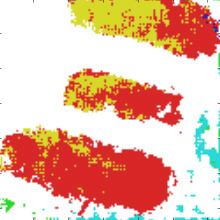
\includegraphics[width=\linewidth]{evolution/rgb_10000} &
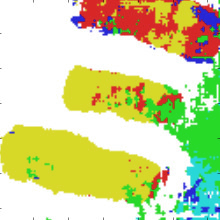
\includegraphics[width=\linewidth]{evolution/rgb_20000} &
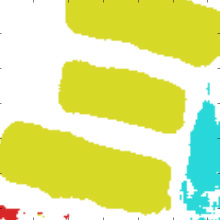
\includegraphics[width=\linewidth]{evolution/rgb_50000} &
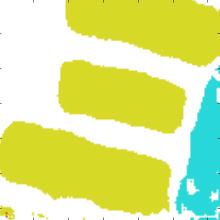
\includegraphics[width=\linewidth]{evolution/rgb_80000} &
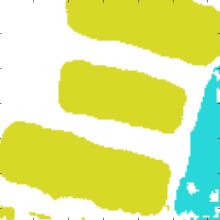
\includegraphics[width=\linewidth]{evolution/rgb_120000} &
RVB &
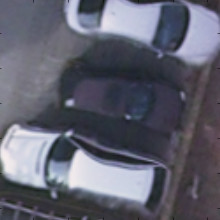
\includegraphics[width=\linewidth]{evolution/rgb} \\
RVB + OSM &
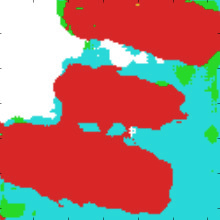
\includegraphics[width=\linewidth]{evolution/osm_10000} &
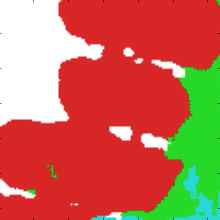
\includegraphics[width=\linewidth]{evolution/osm_20000} &
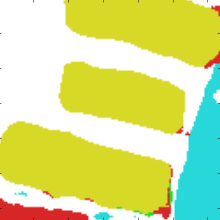
\includegraphics[width=\linewidth]{evolution/osm_50000} &
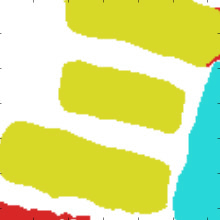
\includegraphics[width=\linewidth]{evolution/osm_80000} &
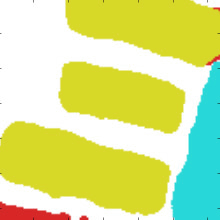
\includegraphics[width=\linewidth]{evolution/osm_120000} &
VT &
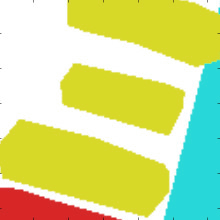
\includegraphics[width=\linewidth]{evolution/gt} \\
itération & 10 000 & 20 000 & 50 000 & 80 000 & 120 000\\
\end{tabularx}
\caption{Évolution des prédictions de SegNet RVB et RBV+OSM. L'ajout de OSM rend les prédictions visuellement plus structurées.
\small{Légende: blanc : routes, \textcolor{Blue}{bleu} : bâtiments, \textcolor{Cerulean}{cyan} : végétation basse, \textcolor{OliveGreen}{vert} : arbres, \textcolor{Dandelion}{jaune} : véhicules, \textcolor{BrickRed}{rouge} : autre}}
\label{fig:training_evolution}
\end{figure}

Par ailleurs, l'intégration des données OSM dans l'apprentissage permet d'accélérer la convergence du modèle. Sur le même jeu de données, le modèle SegNet appris par raffinement depuis OSM nécessite 25\% d'itérations en moins que le SegNet RVB classique et converge vers un meilleur optimal local, avec une fonction de coût à 0,39 contre 0,45, pour un même taux de réussite. Enfin, l'inclusion des données OSM rend la sortie du réseau visuellement plus cohérente et mieux structurée spatialement, comme illustré dans la~\cref{fig:training_evolution}.

Apport sur des classes connues *et* inconnues !

\bibliographystyle{plainnat}
\bibliography{Chapitre4/Biblio}
